\documentclass[]{article}

\usepackage[within=section]{newfloat}
\usepackage{caption}
\usepackage{url}
\usepackage{graphicx}

\DeclareFloatingEnvironment[name=کد,within=none,placement=h]{code}
\captionsetup{belowskip=-10pt,aboveskip=-5pt}

\usepackage{xcolor}
\usepackage[section,newfloat=true]{minted}

\usemintedstyle{manni}

\definecolor{mintedbackground}{rgb}{0.95,0.95,0.95}
\setminted[python]{linenos,breaklines,bgcolor=mintedbackground,frame=leftline,autogobble}
\setminted[bash]{breaklines,bgcolor=mintedbackground,frame=leftline,autogobble}

\usepackage{enumerate}

\usepackage{xepersian}
\settextfont{XB Niloofar}


% Title Page
\title{گزارش پیاده‌سازی الگوریتم‌های \\ \lr{Least Square (closed form)} \\ و \\ \lr{‌Batch Gradient Descent}}
\author{محمد شعاعی}


\begin{document}
\maketitle

\part{توابع و کلاس‌ها}

پیاده سازی الگوریتم‌ها با استفاده از زبان برنامه‌نویسی پایتون\footnote{python} انجام شده است. فایل‌های مربوط به این گزارش عبارتند از:
\begin{enumerate}
	\item \lr{preprocess.py}: این فایل شامل ۲ تابع برای نرمال‌سازی داده و ۱ تابع برای محاسبه خطا است.
	\begin{enumerate}
		\item \lr{\mintinline{python}{zero_mean_normalize(df: pd.DataFrame, columns: list)}}: این تابع ستون‌های مشخص شده را نرمال‌سازی می‌کند. اجرای این تابع داده‌ی اولیه را تغییر می‌دهد.
		
		\item \lr{\mintinline{python}{min_max_normalize(df: pd.DataFrame, columns: list)}}: این تابع با استفاده از روش کمینه-بیشینه داده‌ها را نرمال می‌کند. این تابع داده اولیه را تغییر می‌دهد.
		
		\item \lr{\mintinline{python}{mean_squared_error(y_true, y_pred)}}: این تابع میانگین مربع خطا را به صورت یک عدد اعشاری باز می‌گرداند.
	\end{enumerate}
	
	\item \lr{regressors.py}: این فایل شامل ۳ کلاس مربوط به پیاده سازی الگوریتم های مختلف رگرسیون خطی است.
	\begin{enumerate}
		\item \lr{\mintinline{python}{class LeastSquareRegressor}}: این کلاس شامل پیاده سازی فرم بسته\footnote{closed form} است.
		\item \lr{\mintinline{python}{class BGDRegressor}}: این کلاس شامل پیاده سازی الگوریتم گرادیان کاهشی دسته‌ای\footnote{Batch Gradient Descent} است.
		\item \lr{\mintinline{python}{class SGDRegressor}}: این کلاس شامل پیاده سازی الگوریتم گرادیان کاهشی تصادفی\footnote{Stochastic Gradient Descent} است.
	\end{enumerate}

	\item \lr{main.py}: این فایل که به صورت رابط کاربری متنی پیاده سازی شده است از کلاس‌ها و توابعی که پیش از این معرفی شدند استغاده کرده و اطلاعات مورد نیاز مربوط به داده‌های ورودی را در خروجی استاندارد چاپ می‌کند. همچنین نمودارهای مربوط به هر الگوریتم را به صورت فایل ذخیره می‌کند. نحوه‌ی اجرای این فایل در کد \ref{image:run all} نمایش داده شده است
	\begin{enumerate}
		
	\end{enumerate}
\end{enumerate}

\begin{code}
	\begin{latin}
		\begin{minted}{bash}
			$ python main.py --algo=all --normalize=zero-mean --train=Data-Train.csv --test=Data-Test.csv 
		\end{minted}
	\end{latin}
	\caption{اجرای فایل \lr{main.py}}
	\label{image:run all}
\end{code}
در ادامه دو کلاس فرم بسته و گرادیان کاهشی دسته‌ای توضیح داده خواهند شد. همچنین نمودار های مربوط به عملکرد هر یک نمایش داده می‌شود.

\part{\lr{Least Square (closed form)}}
این الگوریتم توسط کلاس \mintinline{python}{LeastSquareRegressor} پیاده‌سازی شده است. این کلاس شامل متدهای زیر است:
\begin{enumerate}
	\item \lr{\mintinline{python}{fit(self, X, y)}}: با اجرای این متد روند یادگیری مدل آغاز شده و ضرایب مربوط به $\theta$ در متغیر \lr{\mintinline{python}{theta_}} ذخیره می‌شوند.
	\item \lr{\mintinline{python}{predict(self, X)}}: این متد برای استفاده از مدل و پیش‌بینی برچسب کاربرد دارد.
\end{enumerate}

\begin{code}
	\begin{latin}
		\begin{minted}{bash}
			$ python main.py --algo=lstsq --normalize=zero-mean --train=Data-Train.csv --test=Data-Test.csv 
			
			theta: [50.29964125 28.93785624]
			coefs: [28.93785624]
			y-intercept: 50.299641248803006
			MSE (train): 8.328012371573903
			MSE (test): 9.98467535752803
		\end{minted}
	\end{latin}
	\caption{اجرای الگوریتم فرم بسته}
	\label{image:run lstsq}
\end{code}

\begin{figure}
	\centering
	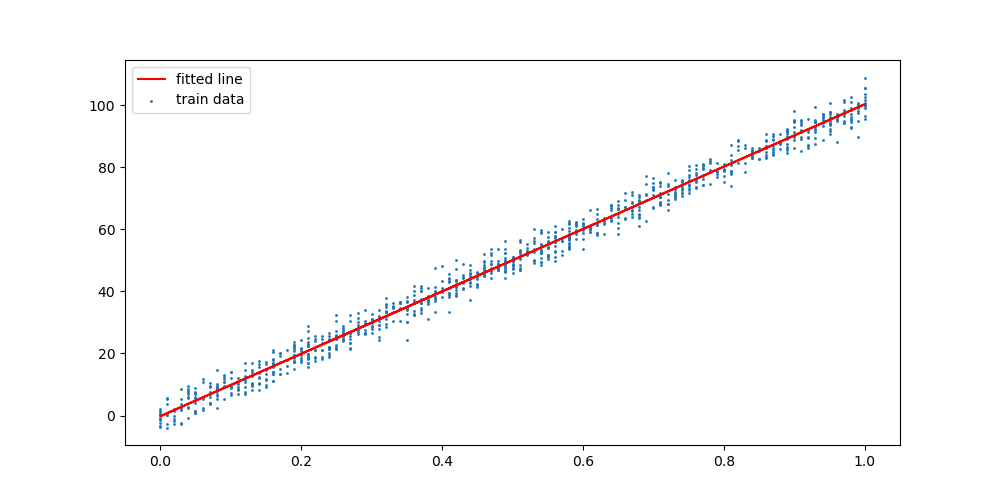
\includegraphics[width=1\linewidth]{lstsq-train}
	\caption{نمودار مربوط به داده \lr{train}}
	\label{fig:lstsq-train}
\end{figure}

\begin{figure}
	\centering
	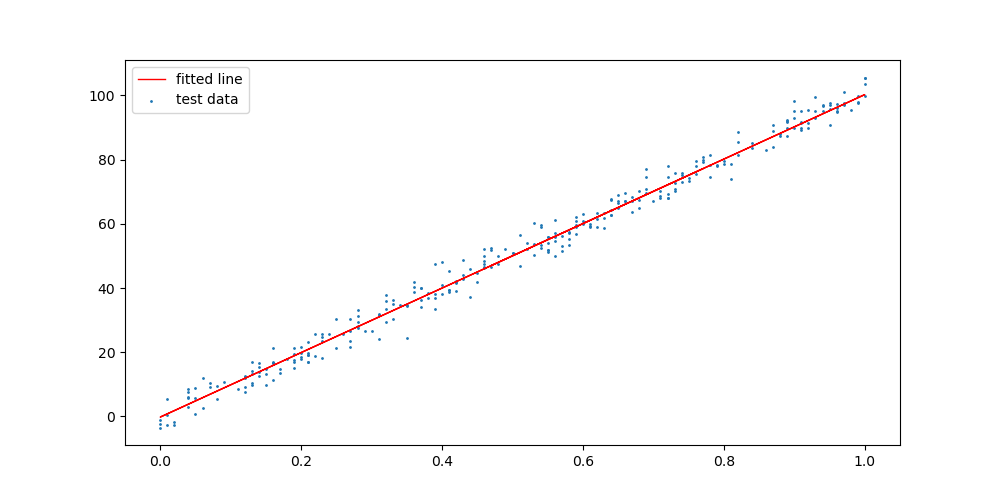
\includegraphics[width=1\linewidth]{lstsq-test}
	\caption{نمودار مربوط به داده \lr{test}}
	\label{fig:lstsq-test}
\end{figure}


\part{\lr{Batch Gradient Descent}}

این الگوریتم با محاسبه‌ی گرادیان مربوط به تمام نمونه‌های موجود و سپس محاسبه‌ی خطا و پس از آن به روزرسانی مفادیر مربوط به $\theta$ اقدام به یافتن خط با کمترین خطا می‌کند. این الگوریتم توسط کلاس \mintinline{python}{BGDRegressor} پیاده‌سازی شده است. این کلاس شامل متدهای زیر است:

\begin{enumerate}
	\item \lr{\mintinline{python}{fit(self, X, y, eta=0.0001, n_iters=1e2)}}: اجرای این متد روند یادگیری مدل را آغاز می‌کند. این متد فرآیند محاسبه‌ی خطا و بروزرسانی $\theta$ را به تعداد \mintinline{python}{n_iter} مرتبه انجام می‌دهد و در هر مرجله مقدار خطا (هزینه) را در متغیر \mintinline{python}{costs_} ذخیره می‌کند.
	\item \lr{\mintinline{python}{predict(self, X)}}: این متد برای استفاده از مدل و پیش‌بینی برچسب .کاربرد دارد
	\item \lr{\mintinline{python}{cost(self, X, y)}}: این متد مقدار هزینه‌ با توجه به $\theta$ فعلی را برمی‌گرداند.
\end{enumerate}

\begin{code}
	\begin{latin}
		\begin{minted}{bash}
			$ python main.py --algo=bgd --normalize=zero-mean --train=Data-Train.csv --test=Data-Test.csv 
			
			theta: [50.29830521996789, 28.93707902574484]
			coefs: [28.93707903]
			y-intercept: 50.29830521996789
			MSE (train): 8.328014760009802
			MSE (test): 9.987058395713497
		\end{minted}
	\end{latin}
	\caption{اجرای الگوریتم گرادیان کاهشی دسته‌ای}
	\label{image:run bgd}
\end{code}
\begin{figure}[h]
	\centering
	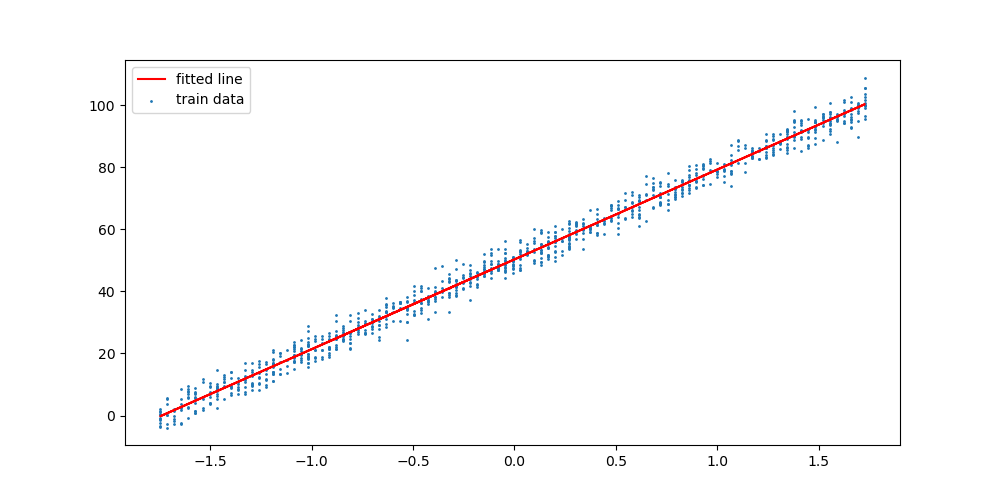
\includegraphics[width=1\linewidth]{bgd-train}
	\caption{نمودار مربوط به داده \lr{train}}
	\label{fig:bgd-train}
\end{figure}
\begin{figure}[h]
	\centering
	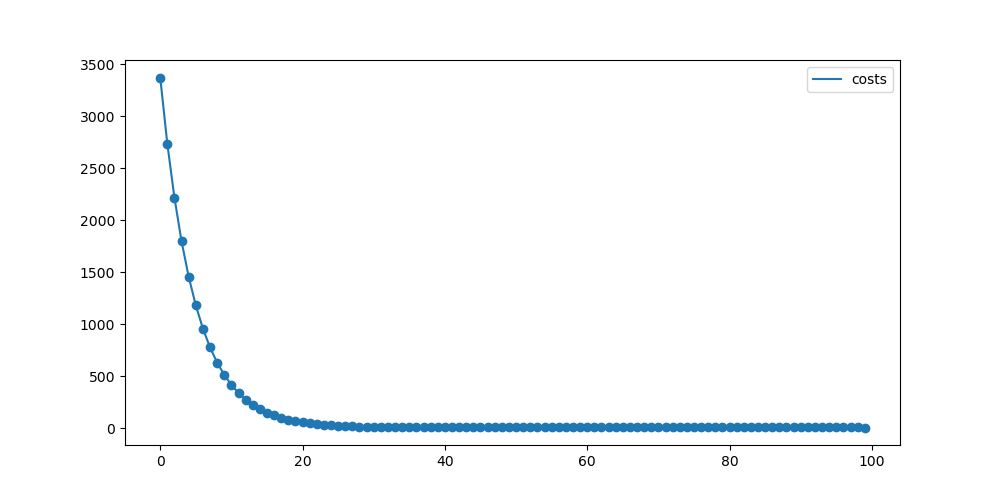
\includegraphics[width=1\linewidth]{bgd-costs}
	\caption{نمودار مربوط به هزینه}
	\label{fig:bgd-costs}
\end{figure}
\begin{figure}[h]
	\centering
	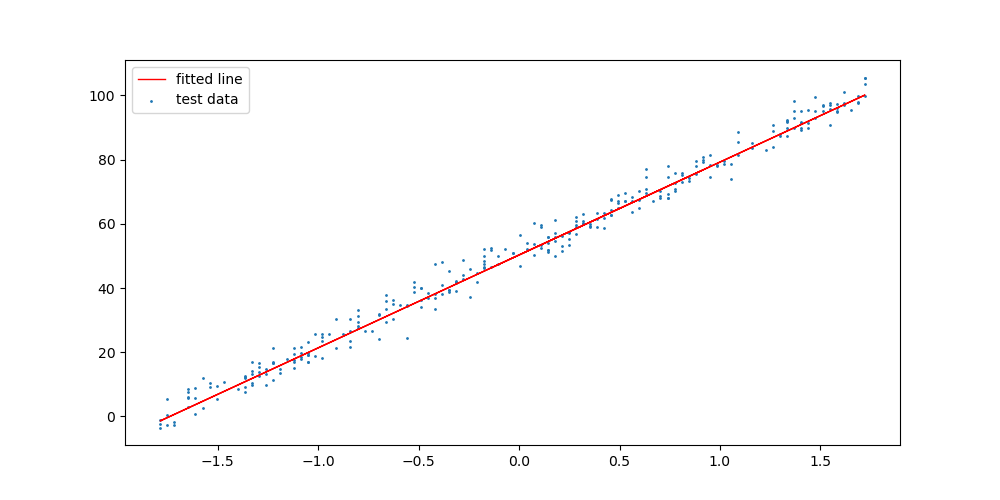
\includegraphics[width=1\linewidth]{bgd-test}
	\caption{نمودار مربوط به داده \lr{test}}
	\label{fig:bgd-test}
\end{figure}

\end{document}
